\section{Experimental Environment}
\label{sec:platform}

	O MPPA é um LW processor desenvolvido pela empresa francesa Kalray. Ele
	é uma das arquiteturas suportadas pelo Nanvix e será utilizado como caso de
	estudo neste trabalho. Conforme a Figura X ilustra, o MPPA integra 288
	núcleos de propósito geral, agrupados em 16 clusters de computação, destinados
	a computação útil, e 4 cluster de IO responsáveis pela comunicação com
	periféricos.  De um lado, cada CC integra 16 PEs, 1 RM, 2~MB de SRAM local,
	duas interfaces NoC e não suportam coerência de cache pelo hardware.  Por outro
	lado, cada IO intergra 4 RMs, 4~MB de SRAM e 8 intefaces NoC. Dois desses IO
	são conectados a um controlador DDR com acesso a 4~GB de DRAM, e os outros dois
	são conectos a controladores Ethernet.  O MPPA também possui duas NoC distintas
	em uma topologia 2-D Torus interpolada, a CNoC e a DNoC. A CNOC é destinada
	a trocas de pequenas mensagens de controle e sincronização e a DNOC é destinada
	a troca de quantidades arbritrárias de dados.

	Figura~\ref{fig:mppa}.
	\begin{figure}[b]
			\centering
			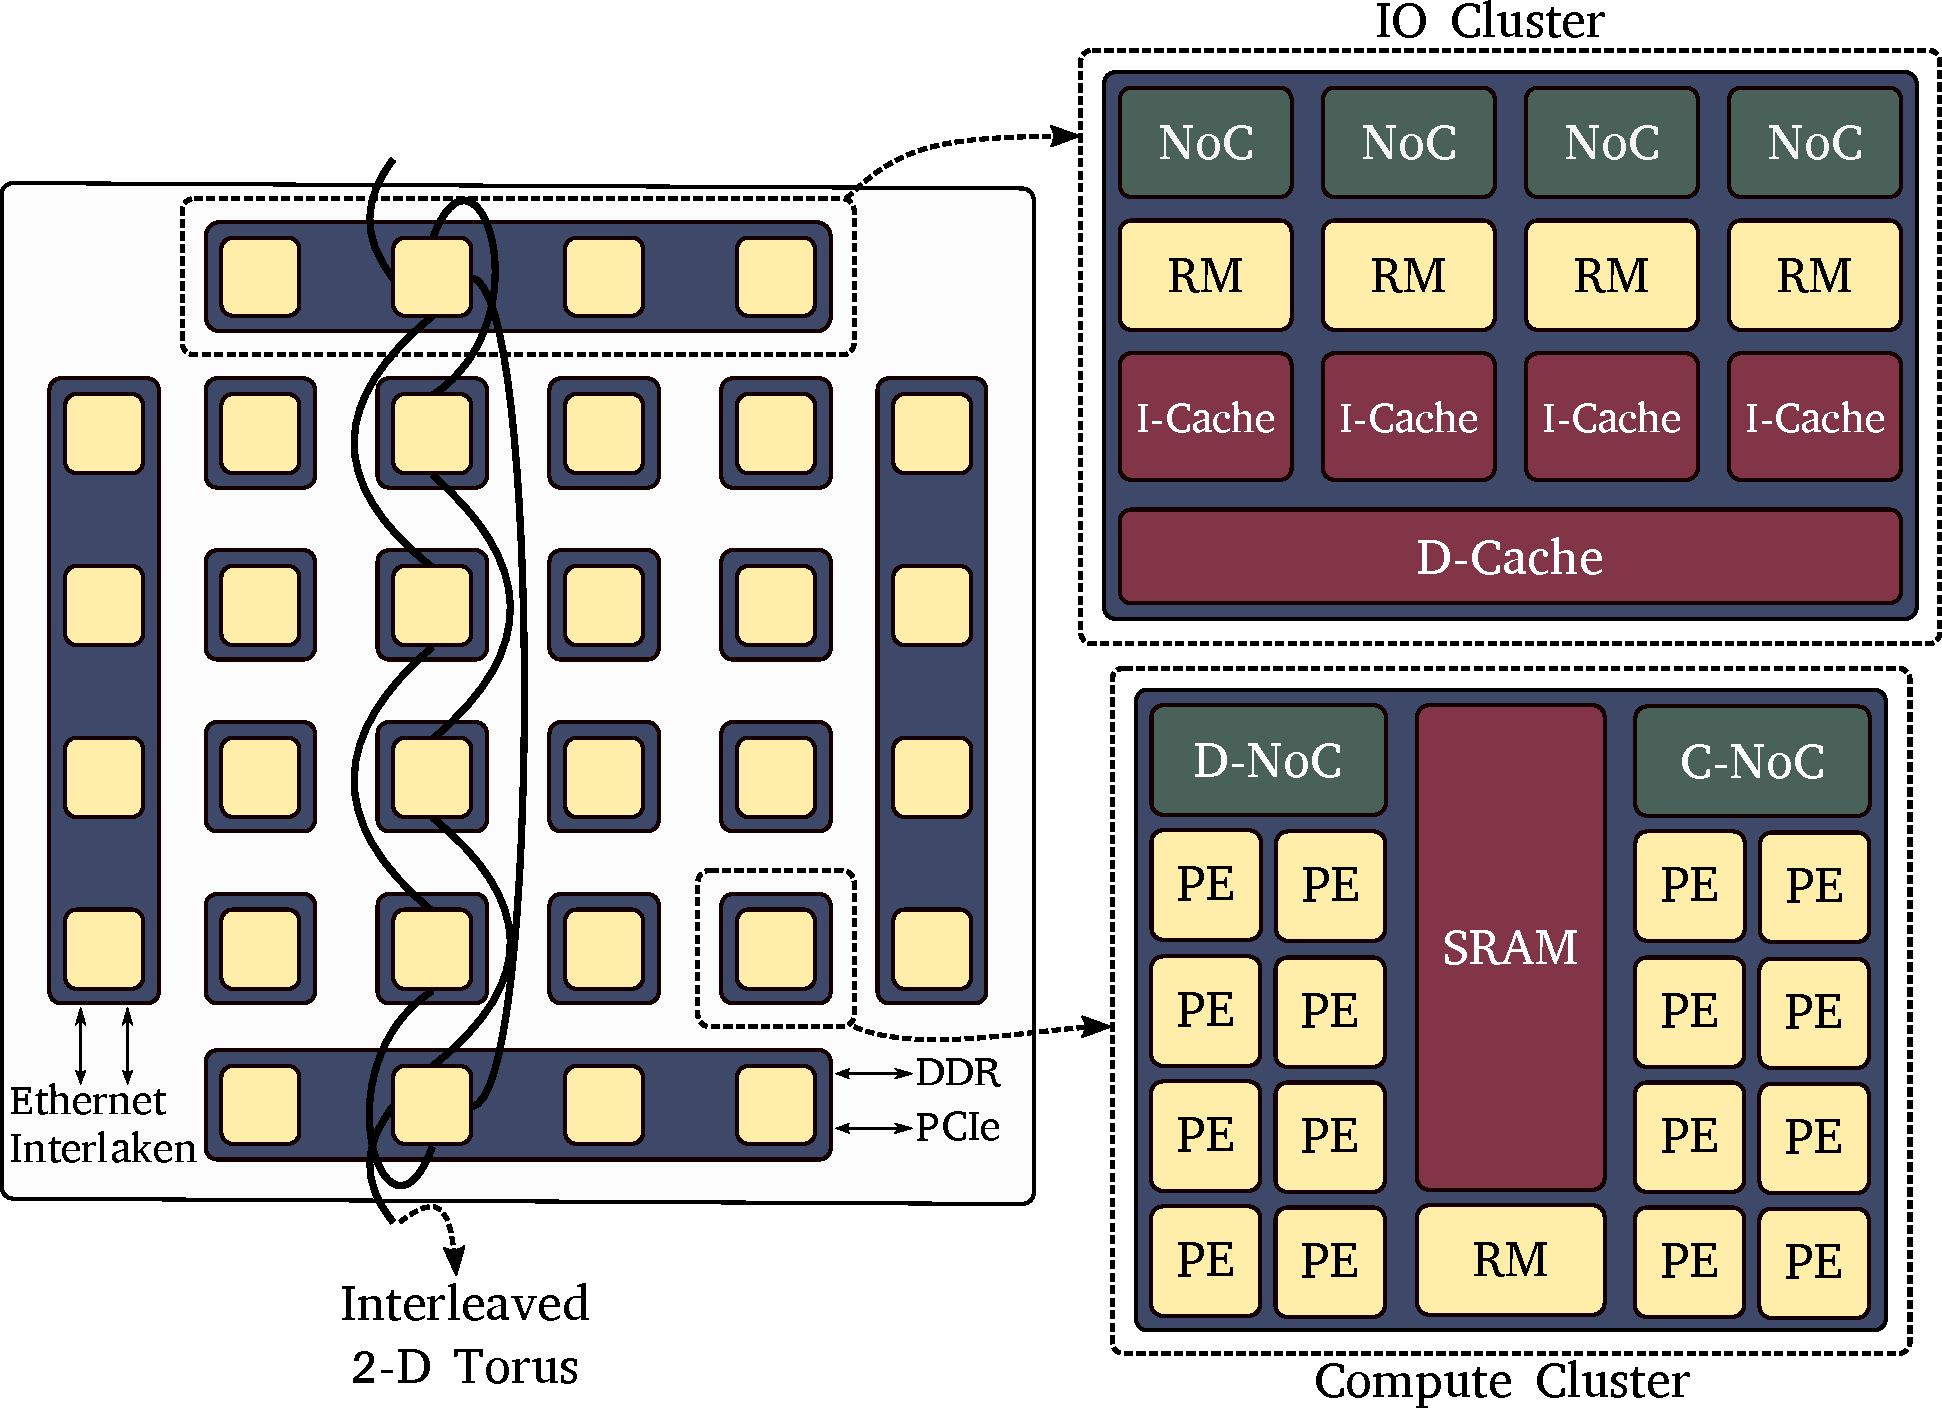
\includegraphics[width=0.90\linewidth]{arch-mppa}
			\caption{\mppa Architecture Overview.}
			\label{fig:mppa}
	\end{figure}


